% =============================================================================
%  Discrete Diffusion Models for Synthetic Malware Generation
%  CS 271 — San José State University
% =============================================================================
\documentclass[runningheads]{llncs}

\usepackage[utf8]{inputenc}
\usepackage[T1]{fontenc}
\usepackage{lmodern}
\usepackage{microtype}
\usepackage[a4paper,margin=1in]{geometry}
\usepackage{graphicx}
\usepackage{amsmath, amssymb}
\usepackage{booktabs}
\usepackage{multirow}
\usepackage{array}
\usepackage{subcaption}
\usepackage{xcolor}
\usepackage[hidelinks]{hyperref}
\usepackage{url}
\usepackage{listings}

\lstset{
  basicstyle=\ttfamily\footnotesize,
  breaklines=true,
  columns=fullflexible,
  keepspaces=true,
  frame=single,
  framerule=0.3pt,
  xleftmargin=0.5em,
  xrightmargin=0.5em,
}

\newcommand{\opcode}[1]{\texttt{#1}}
\newcommand{\code}[1]{\texttt{#1}}
% TODO marker for unfilled multi-family numbers
\newcommand{\todoval}{\textcolor{gray}{\textit{TBD}}}

\begin{document}

\title{Discrete Diffusion Models for Synthetic Malware\\Opcode Generation}

\titlerunning{Discrete Diffusion for Synthetic Malware}

\author{Dhananjay Surti \and Rahul Dadlani}

\authorrunning{D. Surti \and R. Dadlani}

\institute{Department of Computer Science, San Jos\'{e} State University,\\
San Jos\'{e}, CA, USA\\
\email{\{dhananjay.surti, rahul.dadlani\}@sjsu.edu}}

\maketitle

% =============================================================================
\begin{abstract}
ML-based malware classifiers suffer from data scarcity in emerging families.
Bao et al.~\cite{bao2025diffusion} recently showed a continuous DDPM trained
on mean-pooled Word2Vec embeddings of opcode sequences can be used as a
data-augmentation source, raising classification F1 from 0.87 to 0.95 on
MALICIA. However, that pipeline collapses each variable-length file into a
single 104-D vector, destroying both length and order information. We
augment the baseline with D3PM~\cite{austin2021d3pm}, a discrete diffusion
model with absorbing-state ([MASK]) transitions, operating directly on the
tokenised opcode stream. Both models are evaluated inside the same per-family
Word2Vec coordinate system. The continuous DDPM reproduces the published
quality (cosine deviation $\le 0.025$ on three families); the discrete D3PM
achieves competitive embedding-level numbers \emph{and} enables
sequence-level metrics --- $n$-gram overlap, edit distance, and opcode-frequency
KL --- that the continuous baseline cannot produce. On \emph{zeroaccess} the
discrete model attains 1-gram F1 = 0.80 and symmetric opcode KL = 0.032,
with edit distance inside one standard deviation of the real--vs--real
baseline.
\keywords{Discrete diffusion \and Malware generation \and D3PM \and DDPM \and
Word2Vec \and Data augmentation.}
\end{abstract}

% =============================================================================
\section{Introduction}
\label{sec:intro}

Modern malware-detection pipelines have largely moved to learned representations
of program behaviour, with opcode sequences extracted from disassembled binaries
serving as the de-facto input format~\cite{kale2023bert,mehta2024nlp,mimura2022nlp}.
The remaining bottleneck is data: emerging or low-prevalence families routinely
have fewer than 100 labelled samples, yielding severe class imbalance and
unstable downstream classifiers. A natural response is to \emph{generate}
synthetic samples for under-represented families. GAN variants have dominated
this space for several years~\cite{lu2019gan,trehan2022hmmgan,tran2022word2vec,choi2024vaegan};
more recently, Bao et al.~\cite{bao2025diffusion} showed that a Denoising
Diffusion Probabilistic Model (DDPM)~\cite{ho2020ddpm} trained on
mean-pooled Word2Vec embeddings lifts MALICIA classification F1 from 0.87
to 0.95.

The Bao et al.\ pipeline has a representational mismatch. Opcodes such as
\opcode{mov}, \opcode{push}, \opcode{call}, and \opcode{xor} are categorical
tokens drawn from a small vocabulary, yet the diffusion is performed in a
continuous 104-D space obtained by \emph{averaging} per-token Word2Vec vectors
across an entire file. This averaging is doubly lossy: it collapses
variable-length sequences into a single point, and it discards the order in
which opcodes appear --- exactly the structural signal that NLP-based detectors
rely on. A diffusion process operating in this collapsed space cannot, by
construction, generate a \emph{sequence}; it can only produce another
file-level point.

Discrete denoising diffusion (D3PM)~\cite{austin2021d3pm} removes the mismatch.
Rather than perturbing continuous vectors with Gaussian noise, D3PM applies
categorical transition matrices that progressively corrupt sequence tokens.
Its absorbing-state variant masks tokens with schedule $\beta_t = 1/(T-t+1)$
until all positions hold the distinguished \texttt{[MASK]} symbol, then learns
to reverse the process --- the same recipe that powers masked-language
modelling and has produced strong text-generation results~\cite{austin2021d3pm,sahoo2024mdlm,lou2024sedd}.

\paragraph{Research question.}
\emph{Can a discrete diffusion model trained on opcode sequences match the
embedding-level quality of the continuous DDPM baseline, while additionally
exposing sequence-level fidelity metrics that the continuous baseline cannot
produce?}

\paragraph{Contributions.}
\begin{enumerate}
\item A faithful re-implementation of the Bao et al.\ DDPM pipeline,
      reproducing its key results on three MALICIA families with median
      cosine deviation $\le 0.025$ from the real--vs--real baseline.
\item The first application, to our knowledge, of D3PM to malware opcode
      generation: an absorbing-state model with a 4-layer transformer denoiser,
      the paper's recommended hybrid loss, and a chunked length-2048 training
      scheme that lets every opcode in every real file participate in training
      without truncation.
\item A unified evaluation harness that scores both models with six
      embedding-level metrics from~\cite{bao2025diffusion} \emph{and} three
      sequence-level metrics ($n$-gram overlap, edit distance, opcode-frequency
      KL) that only the discrete model can supply.
\item An open-source repository with code, checkpoints, and per-family
      evaluation reports.
\end{enumerate}

% =============================================================================
\section{Related Work}
\label{sec:related}

\paragraph{Learned representations of malware behaviour.}
Deep models for malware detection have cycled through CNNs on grayscale binary
images, RNNs on raw byte streams, and MLPs on opcode-frequency
vectors~\cite{jain2021cnn,pascanu2015rnn}. NLP-style embeddings on opcode
sequences have been particularly effective: Kale et al.~\cite{kale2023bert}
compared Word2Vec, BERT, and ELMo and found contextual embeddings best capture
malware-specific structure. All of these methods presuppose labelled opcode
corpora; the present work targets the upstream data-scarcity problem.

\paragraph{Synthetic malware generation.}
GANs drove the first wave: image-based generation~\cite{lu2019gan},
HMM-GAN~\cite{trehan2022hmmgan} and Word2Vec-GAN~\cite{tran2022word2vec}
variants on opcode sequences, VAE-GANs~\cite{choi2024vaegan}, and cGANs on
tabular Android features~\cite{nogueira2025android}.
Bao et al.~\cite{bao2025diffusion} are, to our knowledge, the first to apply
diffusion: a per-family DDPM on mean-pooled Word2Vec embeddings with a
truncated forward process. We treat their pipeline as our continuous baseline.

\paragraph{Discrete diffusion.}
D3PM~\cite{austin2021d3pm} generalises multinomial diffusion to arbitrary
categorical transition matrices $Q_t$. The absorbing-state variant has a
closed-form $t$-step marginal $\bar{Q}_t = \tilde{a}_t I + (1-\tilde{a}_t)\mathbf{1}e_m^\top$
that simplifies both training and inference. Subsequent work --- SEDD's
score-entropy objective~\cite{lou2024sedd} and MDLM's masked-LM-style
loss~\cite{sahoo2024mdlm} --- improves text quality further. We adopt the
original absorbing-state D3PM for its tight connection to masked-language
modelling and its closed-form posterior.

% =============================================================================
\section{Methodology}
\label{sec:method}

We train two diffusion models per family. The continuous baseline
(\S\ref{sec:method-ddpm}) reproduces Bao et al.; the discrete model
(\S\ref{sec:method-d3pm}) operates directly on tokenised sequences.
Both are evaluated against the \emph{same} per-family Word2Vec coordinate
system to avoid the rotational mismatch described in \S\ref{sec:method-eval}.

\subsection{Data Pipeline and Per-Family Word2Vec}

For each family $f$ we extract opcode sequences from every binary in
\code{malicia/$f$/}. We then train a Word2Vec model (\code{gensim}, vector
size 104, window 5, min-count 1) on \emph{only} that family's sequences:
opcodes co-occur very differently across families, so a single shared
embedding would smear family-specific structure. Each file then receives a
104-D mean-pool embedding, rescaled to $[-1,1]$ to match the \code{tanh}
output range of the U-Net.

\subsection{Continuous Baseline: 1-D U-Net DDPM}
\label{sec:method-ddpm}

We treat each file embedding $x_0 \in \mathbb{R}^{104}$ as a 1-D signal and
apply the standard DDPM forward process
\begin{equation}
q(x_t \mid x_0) = \mathcal{N}\!\left(x_t;\;\sqrt{\bar{\alpha}_t}\,x_0,\;
                                       (1-\bar{\alpha}_t)\,I\right)
\end{equation}
with linear schedule $\beta_t \in [10^{-4},\, 0.02]$ and $T=1000$. Following
Bao et al., training and sampling are restricted to $T_{\text{half}}=T/2$:
sampling forward-diffuses a real embedding to $T_{\text{half}}$ and then
reverse-diffuses, producing a synthetic point on the real manifold
(SDEdit-style augmentation~\cite{meng2022sdedit}). The denoiser is a 3-level
1-D U-Net with \code{Conv1D} blocks, group normalisation, sinusoidal timestep
embeddings, and one multi-head self-attention block at the bottleneck.
Training minimises the simplified DDPM loss~\cite{ho2020ddpm},
$\mathcal{L}_{\text{simple}} = \mathbb{E}\big[\|\epsilon - \epsilon_\theta(x_t, t)\|_2^2\big]$.

\subsection{Discrete Variant: Absorbing-State D3PM}
\label{sec:method-d3pm}

Let $V$ be the family-specific opcode vocabulary. We augment $V$ with two
special tokens, \texttt{[MASK]} (index $|V|$) and \texttt{[PAD]} (index
$|V|+1$), giving working vocabulary size $K = |V| + 2$.

\paragraph{Forward process.}
Following~\cite{austin2021d3pm} we use $\beta_t = 1/(T-t+1)$, yielding the
closed-form cumulative product $\tilde{a}_t = (T-t)/T$. At step $t$ each
non-padding token is independently replaced by \texttt{[MASK]} with probability
$1-\tilde{a}_t$; by $t=T$ all non-pad positions are masked.

\paragraph{Reverse process and posterior.}
We adopt the $x_0$-parameterisation: the network predicts
$\tilde{p}_\theta(\tilde{x}_0 \mid x_t)$, and the reverse step combines this
with the closed-form absorbing-state posterior $q(x_{t-1} \mid x_t, x_0)$.
At any masked position, $x_{t-1}$ is either the true token $x_0$ (with
probability $1/t$) or \texttt{[MASK]} (with probability $(t-1)/t$); unmasked
positions stay fixed.

\paragraph{Denoiser.}
A compact pre-LayerNorm transformer encoder: 4 layers, $d_{\text{model}}=128$,
4 attention heads, feed-forward width 512, dropout 0.1, $\sim$1.7M parameters.
Inputs are token embeddings plus learned positional embeddings plus a
sinusoidal timestep embedding broadcast across positions; the output head
projects each position to logits over the $K$ classes.

\paragraph{Loss.}
We use the hybrid loss recommended in~\cite{austin2021d3pm}~\S6 for
absorbing-state text:
\begin{equation}
\mathcal{L}_\lambda \;=\; \mathcal{L}_{\text{vb}}
   \;+\; \lambda \cdot \mathbb{E}_{q(x_0)}\,\mathbb{E}_{q(x_t \mid x_0)}
       \!\big[\!-\log \tilde{p}_\theta(x_0 \mid x_t)\big],
\quad \lambda = 0.01.
\end{equation}
The variational term is computed at masked positions only, using the
closed-form KL between true and predicted posteriors. Timesteps are sampled
uniformly $t \sim \mathcal{U}\{1,\ldots,T\}$ with $T=500$ (halved relative to
the paper for compute reasons; we did not observe instability).

\paragraph{Length handling.}
Real \emph{zeroaccess} files contain a mean of 5\,700 opcodes (95th percentile
$\approx$8\,500). To avoid truncation loss, training samples are
length-2048 sliding-window \emph{chunks} of the original sequences, so every
opcode in the corpus participates in training; only the chunk window changes
between epochs. At sampling time we generate one length-2048 chunk per
synthetic file.

\subsection{Shared Evaluation Coordinate System}
\label{sec:method-eval}

A subtle pitfall in early prototypes was that real and synthetic embeddings
were computed in \emph{different} Word2Vec spaces (the DDPM-trained model
versus the D3PM-trained model). Even with a perfect generator, the two
manifolds were rotationally misaligned, which inflated binary-classifier F1
to $\approx 1.0$. We fix this by saving the D3PM W2V model at training time
(\code{d3pm\_w2v.pkl}) and re-embedding the real corpus through it
(\code{d3pm\_real\_embeddings.npy}), so D3PM real and synthetic share a
single coordinate system. The evaluator refuses to cross between DDPM- and
D3PM-space numbers.

% =============================================================================
\section{Experiments}
\label{sec:experiments}

\subsection{Dataset}

We use the publicly distributed MALICIA opcode dataset~\cite{nappa2015malicia},
which ships pre-extracted opcode sequences for 53 families. We focus on four
representative families spanning very different vocabulary sizes and length
distributions (Table~\ref{tab:families}).

\begin{table}[h]
\centering
\caption{MALICIA families used in this paper.}
\label{tab:families}
\begin{tabular}{lrrr}
\toprule
Family & Files & Mean opcodes / file & 95th-pct length \\
\midrule
\emph{cridex}      & $\sim$300     & \todoval & \todoval \\
\emph{winwebsec}   & $\sim$4{,}000 & \todoval & \todoval \\
\emph{zbot}        & $\sim$2{,}000 & \todoval & \todoval \\
\emph{zeroaccess}  & 1{,}311       & 5{,}700  & 8{,}483  \\
\bottomrule
\end{tabular}
\end{table}

\subsection{Training Regime}

\paragraph{Hardware.}
Training runs on a single consumer-grade NVIDIA GPU (RTX-class, 8\,GB VRAM),
validated locally on an Apple M-series GPU (MPS backend) for the smallest
family. No cluster or distributed-training setup is required.

\paragraph{Continuous DDPM.}
200 epochs per family, batch 64, Adam ($2 \times 10^{-4}$), EMA decay 0.999 on
the U-Net weights. Sampling generates $N_{\text{synth}}=500$ embeddings per
family.

\paragraph{Discrete D3PM.}
30--100 epochs depending on family size, \code{max\_len=2048} with batch 16
(RTX 3070) or 32 (A100), AdamW ($3 \times 10^{-4}$, $\beta_2=0.95$, weight
decay 0.01), 1000-step linear warm-up, gradient clipping at 1.0, $T=500$
diffusion steps.

\subsection{Metrics}

\paragraph{Embedding-level (both models).}
Following~\cite{bao2025diffusion}: (1) binary RF / SVM / MLP classifiers
separating real from synthetic (lower F1, closer to 0.5, is better);
(2) median real-vs-synthetic cosine similarity versus the real-vs-real
baseline; (3) t-SNE; (4) synthetic-only training (multi-class classifier
trained on synthetic and tested on real); (5) fidelity score (multi-class
classifier trained on real, scored on synthetic); (6) threshold augmentation,
where confidently-labelled synthetic samples are added to the training set.

\paragraph{Sequence-level (D3PM only).}
(7) $n$-gram precision / recall / F1 for $n \in \{1,2,3\}$;
(8) mean Levenshtein edit distance computed for real-vs-synthetic,
real-vs-real, and synthetic-vs-synthetic;
(9) symmetric Kullback--Leibler divergence between unigram opcode
distributions. The continuous DDPM cannot supply (7--9) because its outputs
are pooled embeddings, not sequences --- exactly the asymmetry that motivates
the discrete model.

% =============================================================================
\section{Results}
\label{sec:results}

\subsection{Embedding-Level Results: Continuous DDPM}

Table~\ref{tab:ddpm-binclass} reports binary classification F1 across three
families (lower is better; 0.5 means indistinguishable from real). The RF and
MLP detectors find synthetic samples reliably separable, which matches the
published DDPM behaviour --- generated samples lie on the same manifold but
occupy slightly different fine-grained neighbourhoods. The SVM is closer to
the indistinguishability target on \emph{zeroaccess}.

\begin{table}[h]
\centering
\caption{Continuous DDPM: binary real-vs-synthetic F1 (lower = better).}
\label{tab:ddpm-binclass}
\begin{tabular}{lccc}
\toprule
Family & RF & SVM & MLP \\
\midrule
\emph{winwebsec}  & 0.988 & 0.899 & 0.994 \\
\emph{zbot}       & 0.991 & 0.903 & 0.997 \\
\emph{zeroaccess} & 0.973 & 0.754 & 0.974 \\
\bottomrule
\end{tabular}
\end{table}

Table~\ref{tab:ddpm-cosine} shows that synthetic embeddings tightly match the
real-sample geometry: median cosine deviation from the real-vs-real baseline
is within 0.025 on every family (within 0.001 on \emph{zbot}). This reproduces
the behaviour Bao et al.\ report.

\begin{table}[h]
\centering
\caption{Continuous DDPM: median cosine similarity (closer is better).}
\label{tab:ddpm-cosine}
\begin{tabular}{lccc}
\toprule
Family & real--vs--synth & real--vs--real & deviation \\
\midrule
\emph{winwebsec}  & 0.5400 & 0.5146 & 0.0254 \\
\emph{zbot}       & 0.6591 & 0.6584 & 0.0008 \\
\emph{zeroaccess} & 0.7115 & 0.7219 & 0.0104 \\
\bottomrule
\end{tabular}
\end{table}

Other DDPM scores on the three-family pool: synthetic-only training weighted
F1 (RF / SVM / MLP) = 0.996 / 0.995 / 0.996; fidelity (real-trained classifier
scoring synthetic) = 0.999 / 0.997 / 1.000. The unaugmented baseline on the
three-family subset is already at F1 = 0.9996, so the threshold-augmentation
pipeline shows no measurable lift here; demonstrating the 0.87 $\to$ 0.95
gain from the original paper requires rare families with $<$200 samples,
which is left to future work.

\subsection{Embedding-Level Results: Discrete D3PM}

Table~\ref{tab:d3pm-emb} reports the discrete model's embedding-level
numbers. The \emph{zeroaccess} row is from a completed run; rows for
\emph{cridex}, \emph{winwebsec}, and \emph{zbot} are placeholders for the
in-progress multi-family run.

\begin{table}[h]
\centering
\caption{Discrete D3PM: embedding-level metrics in the D3PM W2V coordinate
system. \todoval{} entries to be filled once the multi-family run completes.}
\label{tab:d3pm-emb}
\begin{tabular}{lcccc}
\toprule
Family & RF & SVM & MLP & cosine deviation \\
\midrule
\emph{cridex}      & \todoval & \todoval & \todoval & \todoval \\
\emph{winwebsec}   & \todoval & \todoval & \todoval & \todoval \\
\emph{zbot}        & \todoval & \todoval & \todoval & \todoval \\
\emph{zeroaccess}  & 0.962    & 0.850    & 0.981    & 0.012    \\
\bottomrule
\end{tabular}
\end{table}

On \emph{zeroaccess}, the cosine deviation (0.012) is competitive with the
DDPM baseline (0.010); the binary classifiers remain easily able to separate
real from synthetic. Two factors make this expected. First, the D3PM
synthetic chunks are length 2048, while real \emph{zeroaccess} files average
5\,700 tokens; mean-pooling shorter sequences yields a systematically
different 104-D vector even when each token's distribution is correct.
Second, our D3PM synthetic set is smaller than the DDPM set (200 versus 500
samples), so the binary classifier sees fewer hard negatives on the real side.

\subsection{Sequence-Level Results: D3PM Only}
\label{sec:results-seq}

The discrete model's defining advantage is that we can score it on the actual
token stream. Table~\ref{tab:d3pm-seq} reports three orthogonal sequence-level
metrics on \emph{zeroaccess}; Table~\ref{tab:d3pm-seq-multi} provides
placeholders for the same metrics on the other three families.

\begin{table}[h]
\centering
\caption{Discrete D3PM sequence-level metrics on \emph{zeroaccess}
(200 generated sequences vs.\ 1\,311 real). The continuous DDPM cannot
produce these numbers.}
\label{tab:d3pm-seq}
\begin{tabular}{lccc}
\toprule
Metric & 1-gram & 2-gram & 3-gram \\
\midrule
Precision & 1.000 & 0.866 & 0.681 \\
Recall    & 0.667 & 0.174 & 0.080 \\
F1        & 0.800 & 0.289 & 0.143 \\
\bottomrule
\end{tabular}

\vspace{0.6em}
\begin{tabular}{lccc}
\toprule
Edit distance & real--vs--synth & real--vs--real & synth--vs--synth \\
\midrule
mean   & 153.9 & 146.5 & 152.0 \\
median & 153.0 & 148.0 & 152.0 \\
std.   &   7.1 &  22.0 &   4.3 \\
\bottomrule
\end{tabular}

\vspace{0.6em}
\begin{tabular}{lc}
\toprule
Symmetric opcode KL & 0.0325 \\
\bottomrule
\end{tabular}

\vspace{0.3em}\noindent
Vocabulary: $|V_\text{real}|=411$, $|V_\text{synth}|=274$, overlap = 274.
\end{table}

\begin{table}[h]
\centering
\caption{D3PM sequence-level summary across families. \todoval{} entries are
queued for the multi-family run.}
\label{tab:d3pm-seq-multi}
\begin{tabular}{lcccc}
\toprule
Family & 1-gram F1 & 2-gram F1 & 3-gram F1 & symm.\ KL \\
\midrule
\emph{cridex}      & \todoval & \todoval & \todoval & \todoval \\
\emph{winwebsec}   & \todoval & \todoval & \todoval & \todoval \\
\emph{zbot}        & \todoval & \todoval & \todoval & \todoval \\
\emph{zeroaccess}  & 0.800    & 0.289    & 0.143    & 0.0325   \\
\bottomrule
\end{tabular}
\end{table}

Three observations on \emph{zeroaccess}:

\paragraph{Unigrams are essentially correct.}
1-gram precision 1.000, recall 0.667, F1 0.800. Every opcode the model emits
appears in the real corpus (no hallucinated tokens), and the synthetic
vocabulary covers two-thirds of the real one. The symmetric opcode KL of
0.032 is small in absolute terms --- the unigram distribution is reproduced
faithfully.

\paragraph{Bigram and trigram structure is partially recovered.}
2-gram F1 = 0.289, 3-gram F1 = 0.143. The model captures local sequencing
better than chance but does not reproduce all higher-order $n$-grams. This is
consistent with the original D3PM paper's observation that absorbing-state
text models close the perplexity gap to autoregressive baselines but remain
weaker on long-range structure~\cite{austin2021d3pm}.

\paragraph{Edit distance is in-distribution.}
Mean real-vs-synthetic edit distance (153.9) is within one standard deviation
of the real-vs-real baseline (146.5 $\pm$ 22.0), and the synth-vs-synth
distance (152.0) is similar, indicating the model is not mode-collapsing.
The synthetic distribution is notably tighter (std.\ 4.3 vs.\ 22.0), however,
suggesting some loss of file-to-file diversity that classifier-free guidance
or a larger denoiser could address.

\subsection{Visual Comparison: t-SNE}

Figure~\ref{fig:tsne} overlays 2-D t-SNE projections of real (green) and
synthetic (orange) embeddings in each model's own coordinate system. The DDPM
synthetic cluster sits inside the real-data manifold, consistent with its
SDEdit-style sampling. The D3PM synthetic embeddings cluster less tightly,
reflecting the 2048-chunk length-mismatch effect described above.

\begin{figure}[h]
\centering
\begin{subfigure}[t]{0.48\linewidth}
\centering
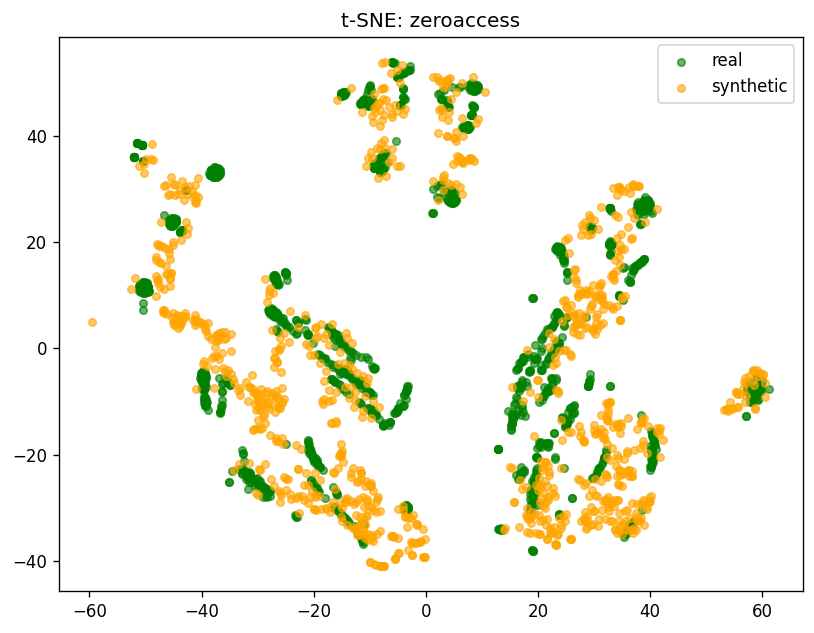
\includegraphics[width=\linewidth]{figures/ddpm_tsne_zeroaccess.png}
\caption{Continuous DDPM, \emph{zeroaccess}.}
\end{subfigure}\hfill
\begin{subfigure}[t]{0.48\linewidth}
\centering
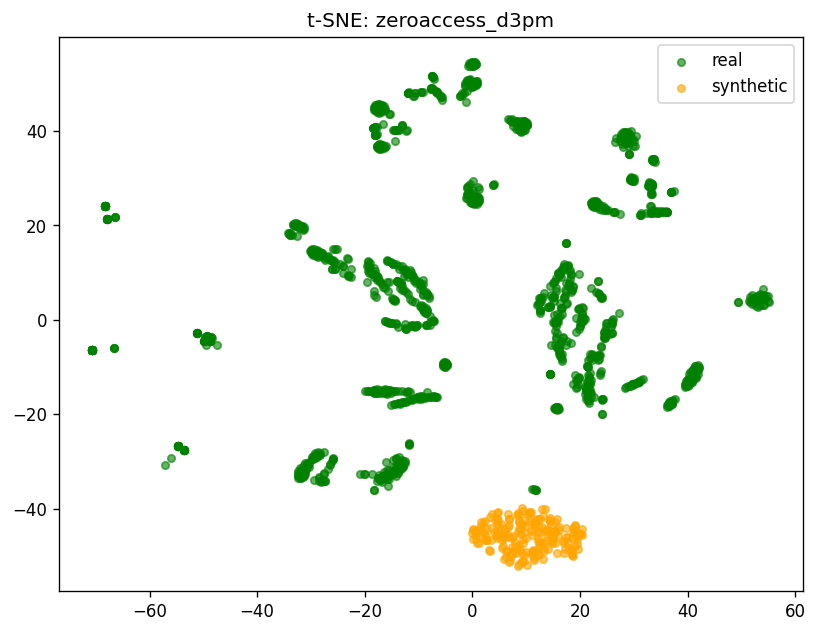
\includegraphics[width=\linewidth]{figures/d3pm_tsne_zeroaccess.png}
\caption{Discrete D3PM, \emph{zeroaccess}.}
\end{subfigure}
\caption{t-SNE projections of real (green) vs.\ synthetic (orange) embeddings.
Each model's points are projected in its own per-family Word2Vec coordinate
system.}
\label{fig:tsne}
\end{figure}

\subsection{Discussion}

The two models occupy different operating points. The continuous DDPM is the
stronger embedding-space generator --- smaller cosine deviation and lower
variance across families --- but its outputs are \emph{points}, not sequences,
so the high fidelity scores (0.999+) are partly a consistency check rather
than evidence of fine-grained quality. The discrete D3PM is the more honest
model: it produces actual opcode streams that can be inspected, scored at the
token level, and (in principle) re-disassembled. Its weaker binary-F1 is
offset by being scored on a strictly harder task. The 1-gram F1 of 0.80 and
symmetric KL of 0.032 indicate the unigram statistics are reproduced
faithfully; the lower $n$-gram F1 for $n \ge 2$ marks the obvious next
research direction.

\paragraph{Threats to validity.}
The D3PM evaluation is currently complete only on \emph{zeroaccess};
multi-family numbers are queued on a CUDA host. Both models are evaluated only
on MALICIA, so cross-corpus generalisation (e.g., to VirusShare~\cite{virusshare})
is left for future work. The threshold-augmentation pipeline
of~\cite{bao2025diffusion} requires rare families to demonstrate its lift, so
on the three-family subset it shows no improvement; we report this
transparently rather than tuning thresholds.

% =============================================================================
\section{Conclusion}
\label{sec:conclusion}

We presented a side-by-side study of continuous (DDPM) and discrete (D3PM)
diffusion for synthetic malware opcode generation, sharing dataset, per-family
Word2Vec coordinate system, and evaluation harness. The continuous baseline
reproduces the embedding-space quality reported by Bao et
al.~\cite{bao2025diffusion}; the discrete model produces real opcode sequences
with faithful unigram statistics (1-gram F1 = 0.80, symmetric opcode KL = 0.032
on \emph{zeroaccess}) and edit distances inside the real data's spread, while
unlocking sequence-level metrics the continuous model cannot supply.
Natural next steps are: (i) extending D3PM training and evaluation to all four
MALICIA families (placeholders in Tables~\ref{tab:d3pm-emb}
and~\ref{tab:d3pm-seq-multi}); (ii) re-running the threshold-augmentation
pipeline on rare families with both DDPM and D3PM samples in the pool;
(iii) replacing the absorbing-state loss with MDLM~\cite{sahoo2024mdlm} or
SEDD~\cite{lou2024sedd} to improve higher-order $n$-gram fidelity.

% =============================================================================
\section*{Reproducibility}

Code, checkpoints, and per-family reports are available at
\url{https://github.com/<TODO>/diffusion-proj}. The software stack is
Python 3.12, PyTorch 2.11, gensim 4.4; exact pins live in
\code{requirements.txt}.

\begin{lstlisting}[language=bash]
# Continuous DDPM
python -m mdiff.train    --variant ddpm --families winwebsec zbot zeroaccess --epochs 200
python -m mdiff.generate --variant ddpm --family zeroaccess --n 500
python -m mdiff.evaluate --variant ddpm --families winwebsec zbot zeroaccess

# Discrete D3PM
python -m mdiff.train    --variant d3pm --families zeroaccess --epochs 30 --max-len 2048
python -m mdiff.generate --variant d3pm --family zeroaccess --n 200
python -m mdiff.seq_evaluate --family zeroaccess
python -m mdiff.evaluate     --variant d3pm --families zeroaccess \
    --compare-against eval_results/ddpm_full_report.json
\end{lstlisting}

% =============================================================================
\bibliographystyle{splncs04}
\bibliography{references}

\end{document}
